% ==============================================================================
% End-to-End System Documentation: MQTT vs LwM2M IoT Firmware Laboratory
% Targets: PC Simulation Environment & STM32 NUCLEO-L452RE-P + Quectel EC200U-CN
% Compile with: pdflatex Firmware_Workflow_Documentation.tex (twice for TOC)
% Compatible with standard TeX Live, MiKTeX, Overleaf
% ==============================================================================
% !TEX program = pdflatex
\documentclass[11pt,a4paper]{article}

\usepackage[T1]{fontenc}
\usepackage[utf8]{inputenc}
\usepackage{lmodern}
\usepackage[margin=2.2cm]{geometry}
\usepackage{xcolor}
\usepackage{booktabs}
\usepackage{tabularx}
\usepackage{longtable}
\usepackage{enumitem}
\usepackage{listings}
\usepackage{tikz}
\usetikzlibrary{arrows.meta,positioning,fit,calc,shapes.geometric}
\usepackage{amsmath,amssymb}
\usepackage[hidelinks]{hyperref}
\usepackage{caption}

% Color definitions
\definecolor{mqttblue}{HTML}{1F618D}
\definecolor{lwm2morange}{HTML}{D35400}
\definecolor{otagreen}{HTML}{117A65}
\definecolor{codebg}{HTML}{F8F9F9}
\definecolor{boxfill}{HTML}{EAECEE}
\definecolor{rulecolor}{HTML}{BDC3C7}

\lstset{
  basicstyle=\ttfamily\footnotesize,
  backgroundcolor=\color{codebg},
  frame=single,
  rulecolor=\color{rulecolor},
  breaklines=true,
  columns=fullflexible,
  keepspaces=true,
  showstringspaces=false,
  xleftmargin=3pt,
  xrightmargin=3pt
}

\newcommand{\code}[1]{\texttt{#1}}
\setlist{itemsep=2pt,topsep=3pt}

\title{\textbf{End-to-End System \& Workflow Documentation}\\[6pt]
\Large Embedded-C IoT Protocol Laboratory and Portable Firmware Architecture\\
\large Detailed Functional Diagrams, Parameter Catalogs, and Execution Workflows for\\
PC Simulation and STM32 NUCLEO-L452RE-P + Quectel EC200U-CN}
\author{IoT Firmware Engineering Team}
\date{October 2026}

\begin{document}

\maketitle

\begin{abstract}
This document provides an exhaustive, end-to-end technical reference for the portable IoT firmware project and protocol evaluation laboratory. The system evaluates two standard telemetry and device-management architectures: \textbf{MQTT} (Eclipse Paho Embedded-C over TCP/TLS) and \textbf{LwM2M} (Eclipse Wakaama over CoAP/UDP/DTLS). It operates across two primary environments: a high-fidelity \textbf{PC Simulation Environment} equipped with a C-based web dashboard host (\code{lab.exe}) and real local/public brokers, and an embedded \textbf{Target Hardware Environment} deploying the exact same core firmware stack to an \textbf{ST NUCLEO-L452RE-P} microcontroller interfaced to a \textbf{Quectel EC200U-CN} LTE Cat-1 cellular modem. This specification documents every functional block, message flow sequence, modem AT state machine, hardware wiring interface, compilation define, and runtime parameter.
\end{abstract}

\tableofcontents
\newpage

% ==============================================================================
\section{Executive Summary and Project Scope}
% ==============================================================================

Modern IoT devices face trade-offs between protocol simplicity (MQTT) and rich device-management capabilities (LwM2M), as well as complex network characteristics across low-bandwidth cellular networks. This project was developed to provide:
\begin{enumerate}
  \item \textbf{High-Fidelity Evaluation Without Hardware Dependencies:} Developers can measure latency, on-the-wire byte overhead, connection setup overhead, and network loss tolerance on a host PC before flashing hardware.
  \item \textbf{100\% Portable Protocol Logic:} The protocol engines (\code{mqtt\_client.c}, \code{lwm2m\_client.c}), telemetry encoding (\code{telemetry.c}), filtering (\code{sensor.c}), and transport security layers (\code{link.c}) are strictly written in C11 and compiled identically on both PC and microcontroller.
  \item \textbf{Drop-in Hardware Portability:} Operating system and peripheral dependencies are decoupled via a thin Platform Abstraction Layer (\code{pal.h} / \code{port.h}). On PC, it interfaces with Winsock/POSIX; on the STM32 target, \code{pal\_ec200u.c} directs data streams through the Quectel EC200U cellular modem's AT command socket stack.
  \item \textbf{Transparent, Empirical Measurements:} Every byte crossing the wire is accounted for (including TCP/IP overhead and TLS/DTLS record envelopes). No simulated metrics are fabricated; missing responses are strictly flagged as failures.
\end{enumerate}

% ==============================================================================
\section{Functional Architecture and System Diagrams}
% ==============================================================================

The system is deployed across two architectural variants: the PC host simulation and the real embedded hardware testbed.

\subsection{PC Simulation Architecture}

In the PC simulation, the complete system runs locally as independent, concurrent C processes communicating over loopback sockets.

\begin{figure}[htbp]
\centering
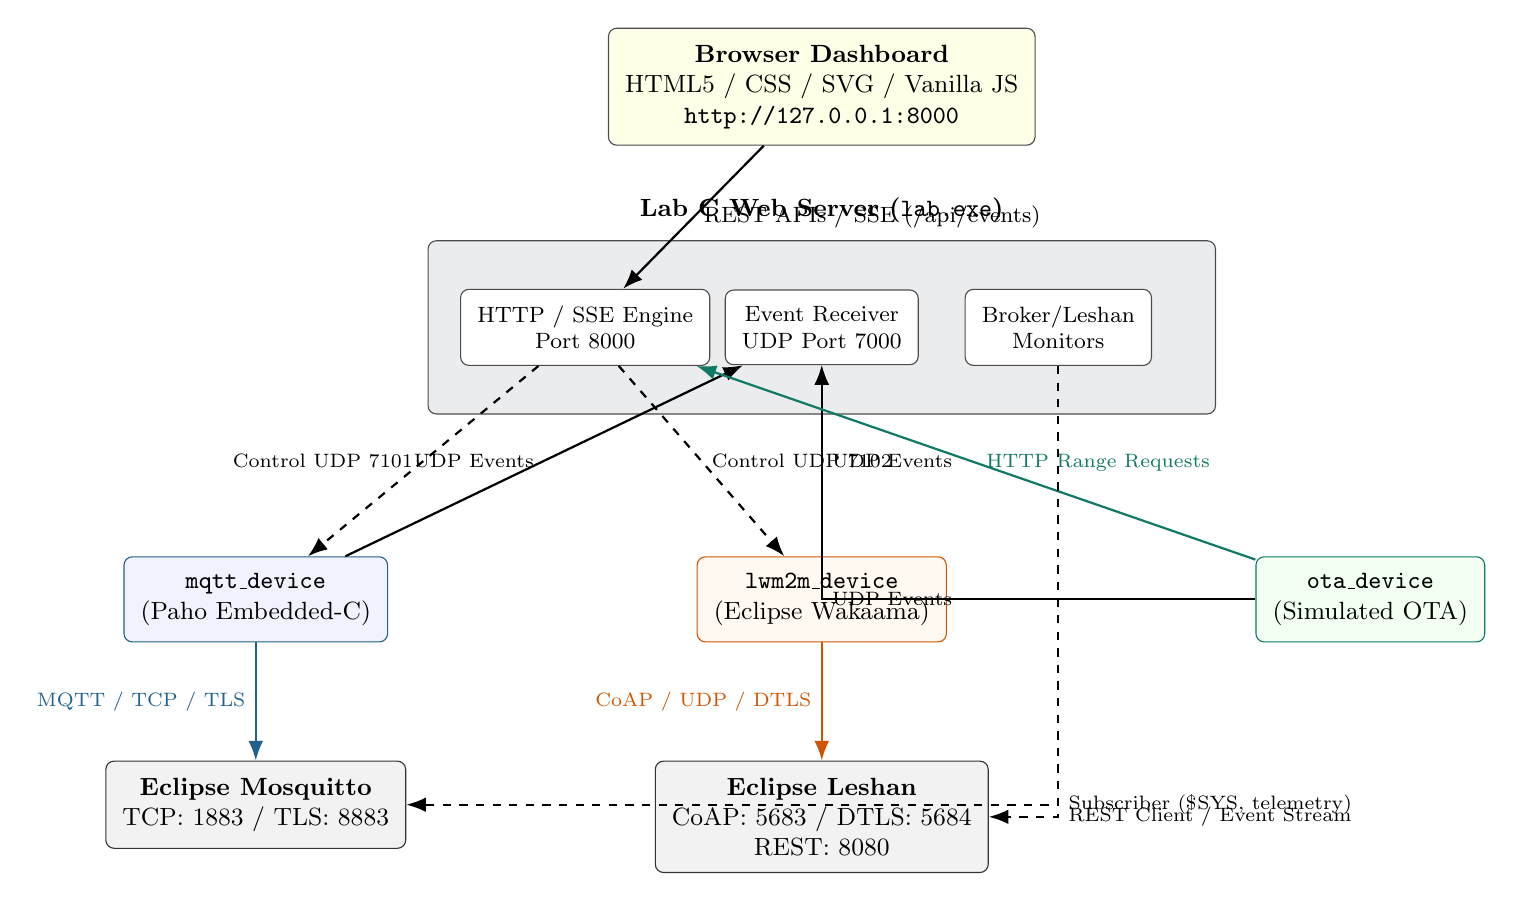
\begin{tikzpicture}[
  box/.style={draw=black!70, fill=boxfill, rounded corners=3pt, align=center, font=\small, inner sep=6pt},
  proc/.style={draw=mqttblue, fill=blue!5, rounded corners=3pt, align=center, font=\small, inner sep=6pt},
  lwmproc/.style={draw=lwm2morange, fill=orange!5, rounded corners=3pt, align=center, font=\small, inner sep=6pt},
  otaproc/.style={draw=otagreen, fill=green!5, rounded corners=3pt, align=center, font=\small, inner sep=6pt},
  server/.style={draw=black!80, fill=gray!10, rounded corners=3pt, align=center, font=\small, inner sep=6pt},
  arr/.style={-{Latex[length=2.5mm]}, thick},
  darr/.style={-{Latex[length=2.5mm]}, dashed, thick}
]

% Nodes
\node[box, fill=yellow!10] (browser) {\textbf{Browser Dashboard}\\HTML5 / CSS / SVG / Vanilla JS\\\code{http://127.0.0.1:8000}};

\node[box, below=1.2cm of browser, minimum width=10cm, minimum height=2.2cm] (lab) {};
\node[above=0.1cm of lab.north, anchor=south, font=\bfseries\small] {Lab C Web Server (\code{lab.exe})};
\node[box, fill=white, font=\footnotesize] at ($(lab.west)!0.2!(lab.east)$) (labhttp) {HTTP / SSE Engine\\Port 8000};
\node[box, fill=white, font=\footnotesize] at ($(lab.west)!0.5!(lab.east)$) (labudp) {Event Receiver\\UDP Port 7000};
\node[box, fill=white, font=\footnotesize] at ($(lab.west)!0.8!(lab.east)$) (labmon) {Broker/Leshan\\Monitors};

\node[proc, below left=1.8cm and 0.5cm of lab] (mqttdev) {\textbf{\code{mqtt\_device}}\\(Paho Embedded-C)};
\node[lwmproc, below=1.8cm of lab] (lwmdev) {\textbf{\code{lwm2m\_device}}\\(Eclipse Wakaama)};
\node[otaproc, below right=1.8cm and 0.5cm of lab] (otadev) {\textbf{\code{ota\_device}}\\(Simulated OTA)};

\node[server, below=1.5cm of mqttdev] (mosq) {\textbf{Eclipse Mosquitto}\\TCP: 1883 / TLS: 8883};
\node[server, below=1.5cm of lwmdev] (lesh) {\textbf{Eclipse Leshan}\\CoAP: 5683 / DTLS: 5684\\REST: 8080};

% Arrows
\draw[arr] (browser) -- node[right, font=\footnotesize] {REST APIs / SSE (/api/events)} (labhttp);
\draw[arr] (mqttdev) -- node[left, font=\scriptsize] {UDP Events} (labudp);
\draw[arr] (lwmdev) -- node[right, font=\scriptsize] {UDP Events} (labudp);
\draw[arr] (otadev) -| node[right, font=\scriptsize] {UDP Events} (labudp);

\draw[darr] (labhttp) -- node[left, font=\scriptsize] {Control UDP 7101} (mqttdev);
\draw[darr] (labhttp) -- node[right, font=\scriptsize] {Control UDP 7102} (lwmdev);

\draw[arr, color=mqttblue] (mqttdev) -- node[left, font=\scriptsize] {MQTT / TCP / TLS} (mosq);
\draw[arr, color=lwm2morange] (lwmdev) -- node[left, font=\scriptsize] {CoAP / UDP / DTLS} (lesh);
\draw[arr, color=otagreen] (otadev) -- node[right, font=\scriptsize] {HTTP Range Requests} (labhttp);

\draw[darr] (labmon) |- node[right, font=\scriptsize] {Subscriber (\$SYS, telemetry)} (mosq);
\draw[darr] (labmon) |- node[right, font=\scriptsize] {REST Client / Event Stream} (lesh);

\end{tikzpicture}
\caption{PC Laboratory Execution and Communication Architecture.}
\label{fig:pc_arch}
\end{figure}

\subsection{Embedded Target Architecture (STM32 Nucleo + EC200U)}

In the hardware configuration, the PC simulated processes are replaced by the \textbf{ST NUCLEO-L452RE-P} microcontroller running \code{pg\_firmware.elf}. The PC continues to run \code{lab.exe}, which communicates bidirectionally over the ST-LINK USB Virtual COM Port (USART2) at 921,600 baud. The STM32 drives the \textbf{Quectel EC200U-CN} modem over USART1 at 115,200 baud through a 1.8V bidirectional level shifter.

\begin{figure}[htbp]
\centering
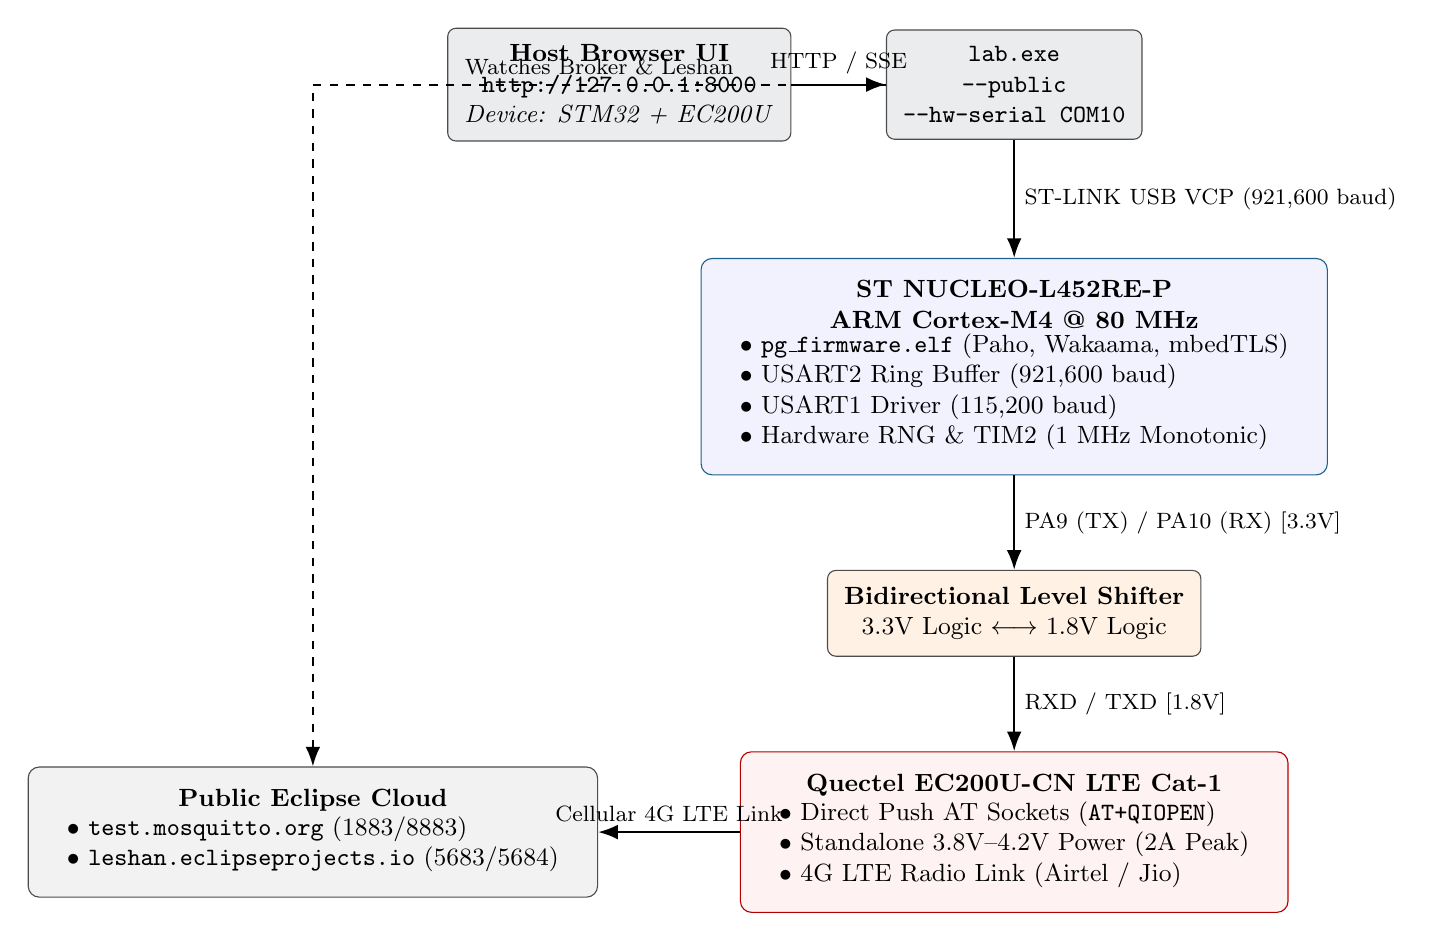
\begin{tikzpicture}[
  box/.style={draw=black!70, fill=boxfill, rounded corners=3pt, align=center, font=\small, inner sep=6pt},
  board/.style={draw=mqttblue, fill=blue!5, rounded corners=4pt, align=center, font=\small, inner sep=8pt},
  modem/.style={draw=red!70!black, fill=red!5, rounded corners=4pt, align=center, font=\small, inner sep=8pt},
  cloud/.style={draw=black!70, fill=gray!10, rounded corners=4pt, align=center, font=\small, inner sep=8pt},
  arr/.style={-{Latex[length=2.5mm]}, thick}
]

\node[box] (ui) {\textbf{Host Browser UI}\\\code{http://127.0.0.1:8000}\\\emph{Device: STM32 + EC200U}};
\node[box, right=1.2cm of ui] (lab) {\textbf{\code{lab.exe}}\\\code{--public}\\\code{--hw-serial COM10}};

\node[board, below=1.5cm of lab] (stm) {\textbf{ST NUCLEO-L452RE-P}\\\textbf{ARM Cortex-M4 @ 80 MHz}\\
  \begin{tabular}{l}
    $\bullet$ \code{pg\_firmware.elf} (Paho, Wakaama, mbedTLS)\\
    $\bullet$ USART2 Ring Buffer (921,600 baud)\\
    $\bullet$ USART1 Driver (115,200 baud)\\
    $\bullet$ Hardware RNG \& TIM2 (1 MHz Monotonic)
  \end{tabular}
};

\node[box, fill=orange!10, below=1.2cm of stm] (shifter) {\textbf{Bidirectional Level Shifter}\\3.3V Logic $\longleftrightarrow$ 1.8V Logic};

\node[modem, below=1.2cm of shifter] (ec200) {\textbf{Quectel EC200U-CN LTE Cat-1}\\
  \begin{tabular}{l}
    $\bullet$ Direct Push AT Sockets (\code{AT+QIOPEN})\\
    $\bullet$ Standalone 3.8V--4.2V Power (2A Peak)\\
    $\bullet$ 4G LTE Radio Link (Airtel / Jio)
  \end{tabular}
};

\node[cloud, left=1.8cm of ec200] (publicservers) {\textbf{Public Eclipse Cloud}\\
  \begin{tabular}{l}
    $\bullet$ \code{test.mosquitto.org} (1883/8883)\\
    $\bullet$ \code{leshan.eclipseprojects.io} (5683/5684)
  \end{tabular}
};

% Connections
\draw[arr] (ui) -- node[above, font=\footnotesize] {HTTP / SSE} (lab);
\draw[arr] (lab) -- node[right, font=\footnotesize] {ST-LINK USB VCP (921,600 baud)} (stm);
\draw[arr] (stm) -- node[right, font=\footnotesize] {PA9 (TX) / PA10 (RX) [3.3V]} (shifter);
\draw[arr] (shifter) -- node[right, font=\footnotesize] {RXD / TXD [1.8V]} (ec200);
\draw[arr] (ec200) -- node[above, font=\footnotesize] {Cellular 4G LTE Link} (publicservers);
\draw[arr, dashed] (lab) -| node[above, near start, font=\footnotesize] {Watches Broker \& Leshan} (publicservers);

\end{tikzpicture}
\caption{Embedded Target (STM32 + EC200U) End-to-End Testbed Architecture.}
\label{fig:stm32_arch}
\end{figure}

\subsection{Firmware Layering and Modularity}

The firmware follows strict layered isolation. High-level layers only invoke functions declared directly below them:

\begin{table}[htbp]
\centering
\small
\begin{tabularx}{\textwidth}{l p{5cm} X}
\toprule
\textbf{Layer} & \textbf{Component Files} & \textbf{Functional Responsibility} \\
\midrule
\textbf{Application} & \code{device.c}, \code{telemetry.c}, \code{sensor.c} & High-level state machine, sampling scheduling, JSON telemetry formatting, and Exponential Moving Average (EMA) filtering ($\alpha=0.3$). \\
\addlinespace
\textbf{Protocol} & \code{protocol\_manager.c}, \code{mqtt\_client.c}, \code{lwm2m\_client.c} & Backend selection, connection state monitoring, exponential reconnect backoff, Paho MQTT packet parsing, and Wakaama CoAP engine. \\
\addlinespace
\textbf{Security} & \code{tls.c}, \code{dtls.c}, \code{tls\_common.c} & TLS 1.3/1.2 client over TCP, DTLS 1.2 PSK over UDP, mbedTLS CTR-DRBG entropy seeding, and certificate chain verification. \\
\addlinespace
\textbf{Network} & \code{network.c}, \code{socket.c}, \code{link.c}, \code{netsim.c} & Generic byte transport interface (\code{fw\_transport\_t}), socket accounting, and synthetic network latency/loss delay lines. \\
\addlinespace
\textbf{HAL} & \code{timer.c}, \code{storage.c}, \code{power.c} & Wrap-safe deadline software timers, CRC32-validated key-value persistent storage (\code{"FWST"}), and battery voltage scaling. \\
\addlinespace
\textbf{Platform (PAL)} & \code{pal.c} (PC), \code{pal\_ec200u.c} (Board), \code{port\_stm32.c} & Operating system abstraction: monotonic microsecond clocks, sleep, and physical/AT socket dispatch. \\
\bottomrule
\end{tabularx}
\caption{Modular Firmware Layer Structure.}
\label{tab:firmware_layers}
\end{table}

% ==============================================================================
\section{Hardware Architecture and Interface Specifications}
% ==============================================================================

\subsection{Electrical Wiring and Pinout Mapping}

The target hardware configuration couples an ST NUCLEO-L452RE-P development board to a Quectel EC200U-CN breakout board.

\begin{table}[htbp]
\centering
\small
\begin{tabularx}{\textwidth}{l l l l X}
\toprule
\textbf{Nucleo Pin} & \textbf{STM32 Alternate Fn} & \textbf{EC200U Pin} & \textbf{Logic Level} & \textbf{Wiring \& Circuit Instructions} \\
\midrule
\textbf{PA9} (D8) & \code{USART1\_TX} (AF7) & \code{RXD} & 1.8V Domain & \textbf{Level Shift Required:} Connect Nucleo 3.3V TX to high side; shift down to 1.8V modem RX. \\
\addlinespace
\textbf{PA10} (D2) & \code{USART1\_RX} (AF7) & \code{TXD} & 1.8V Domain & \textbf{Level Shift Required:} Connect modem 1.8V TX to low side; shift up to 3.3V Nucleo RX. \\
\addlinespace
\textbf{PA0} (A0) & GPIO Output & \code{PWRKEY} & Open Drain & Pulsed active LOW for 1,250~ms only if the modem fails to respond to initial \code{AT}. \\
\addlinespace
\textbf{PA1} (A1) & GPIO Output & \code{RESET} & Active Low & Optional hardware reset pin (reserved). \\
\addlinespace
\textbf{PA2 / PA3} & \code{USART2\_TX / RX} & ST-LINK MCU & 3.3V CMOS & Virtual COM Port (USB) routed directly to Host PC at 921,600 baud. \\
\addlinespace
\textbf{GND} & Ground & \code{GND} & 0V Reference & Must be tied together across Nucleo, Level Shifter, and Modem board. \\
\addlinespace
\textbf{External DC} & N/A & \code{VBAT} & 3.8V--4.2V & \textbf{Mandatory 2A Peak Supply:} Cellular bursts exceed USB current limits. \\
\bottomrule
\end{tabularx}
\caption{Electrical Wiring Matrix between NUCLEO-L452RE-P and Quectel EC200U-CN.}
\label{tab:wiring}
\end{table}

\subsection{Microcontroller Clocks and Peripherals}
\begin{itemize}
  \item \textbf{System Clock (SYSCLK):} Configured to 80~MHz using the internal Multi-Speed Oscillator (MSI @ 4~MHz) driven through Phase-Locked Loop (PLL) parameters: $M=1, N=40, R=2$.
  \item \textbf{True Random Number Generator (RNG):} Sourced via the dedicated 48~MHz internal oscillator (\code{HSI48}), supplying hardware entropy to mbedTLS via \code{mbedtls\_hardware\_poll()}.
  \item \textbf{High-Resolution Monotonic Timer (TIM2):} Configured as a 32-bit hardware timer running at 1~MHz (prescaler = 79), providing microsecond timestamps (\code{pal\_now\_us()}) that do not drift.
  \item \textbf{Cellular UART (USART1):} Configured to 115,200 baud, 8N1. Serviced by an interrupt-driven 8,192-byte ring buffer in SRAM to prevent overrun during cellular data bursts.
  \item \textbf{Lab Link UART (USART2):} Configured to 921,600 baud, 8N1. High throughput ensures ~1~KB JSON event strings transfer in under 11~ms, preserving real-time protocol timings.
\end{itemize}

\subsection{Memory Allocations and Static Budgets}
The NUCLEO-L452RE-P provides 512~KiB Flash and 160~KiB SRAM. To fit the dual protocol stacks, buffers were optimized:
\begin{itemize}
  \item \textbf{Flash Utilization:} Approximately 290~KiB (including mbedTLS crypto, Paho, Wakaama, and embedded PEM certificates).
  \item \textbf{SRAM Static Footprint:} Approximately 80~KiB allocated to static ring buffers, leaving 80~KiB for RTOS/C-runtime stacks and dynamic heap.
  \item \textbf{Buffer Trimming:} The PC's 20~KiB \code{MQTT\_BUF\_SIZE} was reduced to 4,096 bytes; the Wakaama RX buffer is set to 2,048 bytes; the network queue depth is set to 32 slots.
\end{itemize}

% ==============================================================================
\section{Modem Interface and AT State Machine}
% ==============================================================================

On the STM32 target, \code{ec200u.c} implements a robust finite state machine to manage power, cellular network registration, and socket handling.

\subsection{Modem Bring-Up Sequence}
\begin{enumerate}
  \item \textbf{AT Handshake:} Transmits \code{AT\textbackslash r\textbackslash n} every 500~ms. If no response is received within 3~seconds, \code{PA0} (PWRKEY) is pulled active-low for 1,250~ms to cycle power, followed by a 30-second boot poll.
  \item \textbf{Base Configuration:}
    \begin{itemize}
      \item \code{ATE0}: Disables command echo.
      \item \code{AT+CMEE=2}: Enables verbose error reporting.
      \item \code{AT+QURCCFG="urcport","uart1"}: Routes Unsolicited Result Codes (URCs) to USART1 instead of USB.
      \item \code{AT+QICFG="dataformat",0,0}: Sets raw binary mode for socket transfers.
      \item \code{AT+QISDE=0}: Disables echoed send data during socket writes.
    \end{itemize}
  \item \textbf{SIM and Radio Verification:} Polls \code{AT+CPIN?} until \code{READY} (timeout 10~s). Polls \code{AT+CEREG?} until status indicates Home Network (1) or Roaming (5) (timeout 180~s).
  \item \textbf{PDP Context Activation:} Configures APN via \code{AT+QICSGP=1,1,"<APN>","","",1}. Activates context via \code{AT+QIACT=1} (timeout 150~s). Extracts assigned local IPv4 address.
\end{enumerate}

\subsection{AT Socket Lifecycle (Direct Push Mode)}
To preserve compatibility with the PC's BSD socket interface, sockets are configured in Direct Push mode:
\begin{itemize}
  \item \textbf{Connect:} Executes \code{AT+QIOPEN=1,<id>,"TCP"|"UDP","<host>",<port>,0,1}. Waits for URC \code{+QIOPEN: <id>,0}.
  \item \textbf{Transmit:} Executes \code{AT+QISEND=<id>,<len>}. Waits for the prompt character \code{>}. Emits binary payload. Awaits confirmation \code{SEND OK}. Packets exceeding 1,460 bytes are segmented automatically.
  \item \textbf{Receive:} When data arrives, the modem emits \code{+QIURC: "recv",<id>,<len>} followed immediately by the raw byte stream. The interrupt service routine reads these bytes directly from the UART into the socket's internal FIFO ring buffer.
  \item \textbf{Close:} Executes \code{AT+QICLOSE=<id>,10}.
\end{itemize}

% ==============================================================================
\section{Protocol Workflows and Sequence Diagrams}
% ==============================================================================

\subsection{MQTT End-to-End Session Workflow}

\begin{figure}[htbp]
\centering
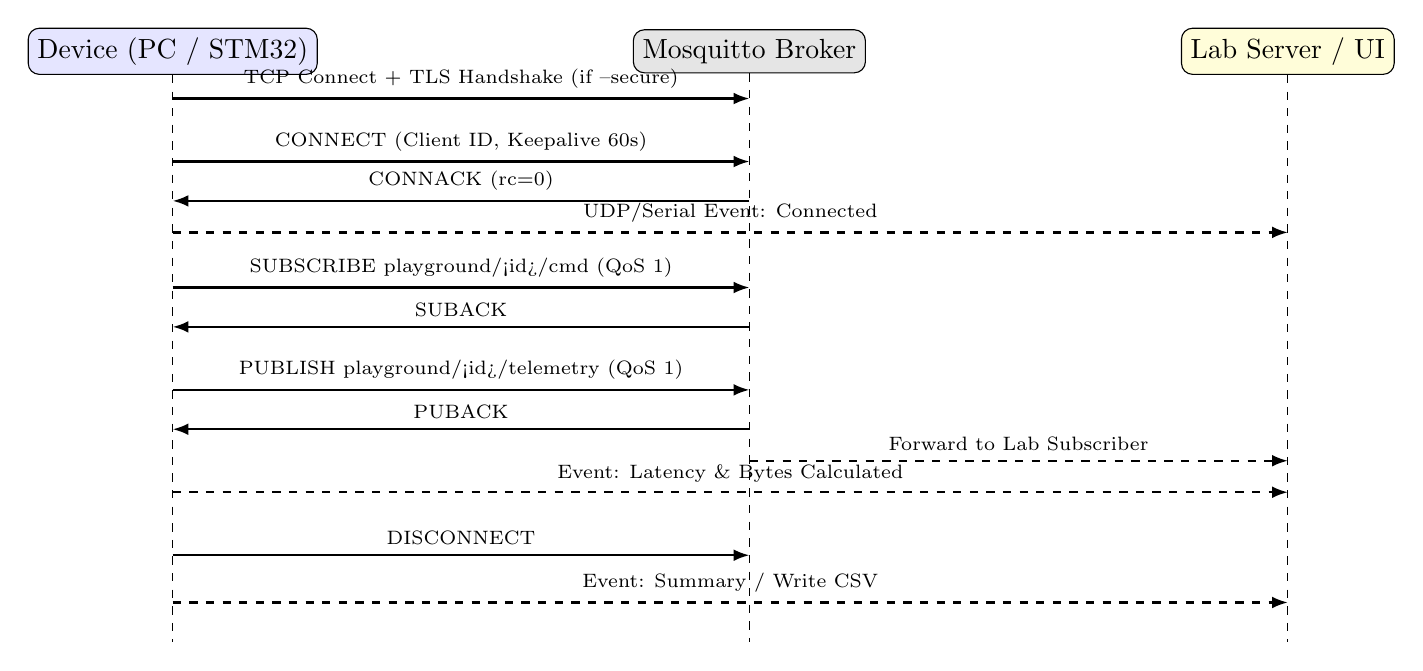
\begin{tikzpicture}[
  node distance=1.5cm,
  line/.style={draw, -{Latex[length=2mm]}, thick},
  msg/.style={font=\scriptsize, align=center}
]
\node[draw, fill=blue!10, rounded corners] (dev) {Device (PC / STM32)};
\node[draw, fill=gray!20, rounded corners, right=4cm of dev] (broker) {Mosquitto Broker};
\node[draw, fill=yellow!15, rounded corners, right=4cm of broker] (lab) {Lab Server / UI};

% Lifelines
\draw[dashed] (dev) -- ++(0,-7.5);
\draw[dashed] (broker) -- ++(0,-7.5);
\draw[dashed] (lab) -- ++(0,-7.5);

% Messages
\draw[line] ($(dev)+(0,-0.6)$) -- node[above, msg] {TCP Connect + TLS Handshake (if --secure)} ($(broker)+(0,-0.6)$);
\draw[line] ($(dev)+(0,-1.4)$) -- node[above, msg] {CONNECT (Client ID, Keepalive 60s)} ($(broker)+(0,-1.4)$);
\draw[line] ($(broker)+(0,-1.9)$) -- node[above, msg] {CONNACK (rc=0)} ($(dev)+(0,-1.9)$);
\draw[line, dashed] ($(dev)+(0,-2.3)$) -- node[above, msg] {UDP/Serial Event: Connected} ($(lab)+(0,-2.3)$);

\draw[line] ($(dev)+(0,-3.0)$) -- node[above, msg] {SUBSCRIBE playground/<id>/cmd (QoS 1)} ($(broker)+(0,-3.0)$);
\draw[line] ($(broker)+(0,-3.5)$) -- node[above, msg] {SUBACK} ($(dev)+(0,-3.5)$);

\draw[line] ($(dev)+(0,-4.3)$) -- node[above, msg] {PUBLISH playground/<id>/telemetry (QoS 1)} ($(broker)+(0,-4.3)$);
\draw[line] ($(broker)+(0,-4.8)$) -- node[above, msg] {PUBACK} ($(dev)+(0,-4.8)$);
\draw[line, dashed] ($(broker)+(0,-5.2)$) -- node[above, msg] {Forward to Lab Subscriber} ($(lab)+(0,-5.2)$);
\draw[line, dashed] ($(dev)+(0,-5.6)$) -- node[above, msg] {Event: Latency \& Bytes Calculated} ($(lab)+(0,-5.6)$);

\draw[line] ($(dev)+(0,-6.4)$) -- node[above, msg] {DISCONNECT} ($(broker)+(0,-6.4)$);
\draw[line, dashed] ($(dev)+(0,-7.0)$) -- node[above, msg] {Event: Summary / Write CSV} ($(lab)+(0,-7.0)$);

\end{tikzpicture}
\caption{MQTT Telemetry Session Sequence.}
\label{fig:seq_mqtt}
\end{figure}

\subsection{LwM2M End-to-End Session Workflow}

\begin{figure}[htbp]
\centering
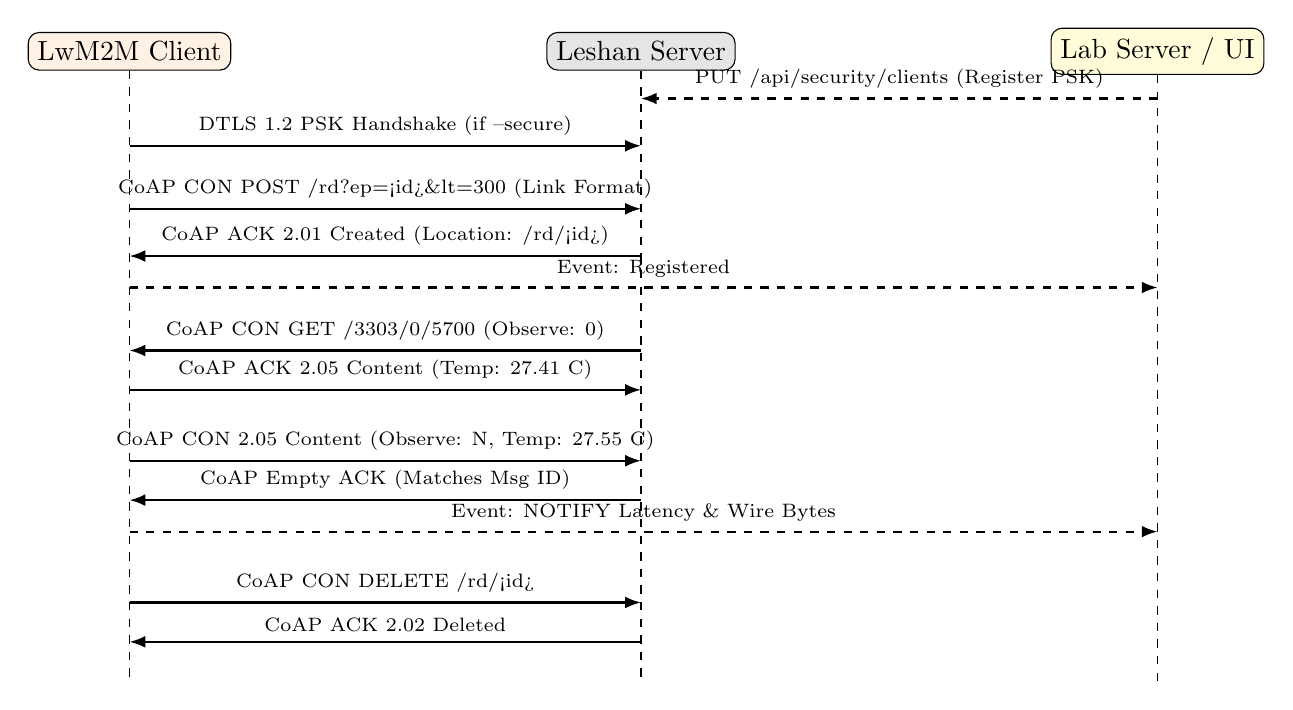
\begin{tikzpicture}[
  node distance=1.5cm,
  line/.style={draw, -{Latex[length=2mm]}, thick},
  msg/.style={font=\scriptsize, align=center}
]
\node[draw, fill=orange!10, rounded corners] (dev) {LwM2M Client};
\node[draw, fill=gray!20, rounded corners, right=4cm of dev] (server) {Leshan Server};
\node[draw, fill=yellow!15, rounded corners, right=4cm of server] (lab) {Lab Server / UI};

% Lifelines
\draw[dashed] (dev) -- ++(0,-8.0);
\draw[dashed] (server) -- ++(0,-8.0);
\draw[dashed] (lab) -- ++(0,-8.0);

% Messages
\draw[line, dashed] ($(lab)+(0,-0.6)$) -- node[above, msg] {PUT /api/security/clients (Register PSK)} ($(server)+(0,-0.6)$);
\draw[line] ($(dev)+(0,-1.2)$) -- node[above, msg] {DTLS 1.2 PSK Handshake (if --secure)} ($(server)+(0,-1.2)$);

\draw[line] ($(dev)+(0,-2.0)$) -- node[above, msg] {CoAP CON POST /rd?ep=<id>\&lt=300 (Link Format)} ($(server)+(0,-2.0)$);
\draw[line] ($(server)+(0,-2.6)$) -- node[above, msg] {CoAP ACK 2.01 Created (Location: /rd/<id>)} ($(dev)+(0,-2.6)$);
\draw[line, dashed] ($(dev)+(0,-3.0)$) -- node[above, msg] {Event: Registered} ($(lab)+(0,-3.0)$);

\draw[line] ($(server)+(0,-3.8)$) -- node[above, msg] {CoAP CON GET /3303/0/5700 (Observe: 0)} ($(dev)+(0,-3.8)$);
\draw[line] ($(dev)+(0,-4.3)$) -- node[above, msg] {CoAP ACK 2.05 Content (Temp: 27.41 C)} ($(server)+(0,-4.3)$);

\draw[line] ($(dev)+(0,-5.2)$) -- node[above, msg] {CoAP CON 2.05 Content (Observe: N, Temp: 27.55 C)} ($(server)+(0,-5.2)$);
\draw[line] ($(server)+(0,-5.7)$) -- node[above, msg] {CoAP Empty ACK (Matches Msg ID)} ($(dev)+(0,-5.7)$);
\draw[line, dashed] ($(dev)+(0,-6.1)$) -- node[above, msg] {Event: NOTIFY Latency \& Wire Bytes} ($(lab)+(0,-6.1)$);

\draw[line] ($(dev)+(0,-7.0)$) -- node[above, msg] {CoAP CON DELETE /rd/<id>} ($(server)+(0,-7.0)$);
\draw[line] ($(server)+(0,-7.5)$) -- node[above, msg] {CoAP ACK 2.02 Deleted} ($(dev)+(0,-7.5)$);

\end{tikzpicture}
\caption{LwM2M Registration, Observation, and Notification Sequence.}
\label{fig:seq_lwm2m}
\end{figure}

\subsection{Simulated Over-The-Air (OTA) Update Workflow}
The OTA mechanism models firmware distribution without requiring custom flash layouts:
\begin{enumerate}
  \item \textbf{Manifest Retrieval:} The device executes an HTTP GET to \code{/ota/manifest?image=<name>}, receiving a JSON object containing target image size and SHA-256 digest.
  \item \textbf{Chunked Range Downloads:} The client issues segmented HTTP Range requests (\code{Range: bytes=offset-(offset+chunk-1)}), saving chunks to \code{results/ota\_storage/slot\_b.bin}. Failed chunks are retried up to 3 times.
  \item \textbf{Integrity Verification:} The device computes the SHA-256 hash over the downloaded file. If it matches the manifest, \code{active\_version.txt} is updated; otherwise, the download is aborted.
\end{enumerate}

% ==============================================================================
\section{Comprehensive Parameter Catalog}
% ==============================================================================

This catalog defines every parameter in the codebase, detailing its default value, valid range, and configuration point.

\subsection{Build-Time CMake and Preprocessor Definitions}

\begin{longtable}{p{4.5cm} p{2.2cm} p{3.5cm} p{5cm}}
\toprule
\textbf{Parameter Macro} & \textbf{Default} & \textbf{Range / Options} & \textbf{Description \& Configuration Point} \\
\midrule
\endfirsthead
\toprule
\textbf{Parameter Macro} & \textbf{Default} & \textbf{Range / Options} & \textbf{Description \& Configuration Point} \\
\midrule
\endhead
\bottomrule
\endfoot
\code{FW\_PLATFORM} & \code{"pc"} & \code{"pc"}, \code{"stm32"} & CMake cache variable: \code{-DFW\_PLATFORM=pc}. Selects platform directory. \\
\addlinespace
\code{FW\_PROTOCOL} & \code{0} (MQTT) & \code{0} (MQTT), \code{1} (LwM2M) & Set in \code{fw\_config.h}. Selects default compile-time protocol. \\
\addlinespace
\code{FW\_USE\_MBEDTLS} & \code{ON} & \code{ON}, \code{OFF} & CMake option. Controls mbedTLS library compilation. \\
\addlinespace
\code{FW\_USE\_PAHO} & \code{ON} & \code{ON}, \code{OFF} & CMake option. Enables Paho Embedded-C packet parser. \\
\addlinespace
\code{FW\_USE\_WAKAAMA} & \code{ON} & \code{ON}, \code{OFF} & CMake option. Enables Eclipse Wakaama LwM2M client. \\
\addlinespace
\code{FW\_MQTT\_HOST} & \code{"test.mosquitto.org"} & Hostname / IPv4 & Build-time default MQTT broker address. \\
\addlinespace
\code{FW\_MQTT\_USE\_TLS} & \code{0} & \code{0} (Plain), \code{1} (TLS) & Build-time flag toggling TLS encryption for MQTT. \\
\addlinespace
\code{FW\_MQTT\_PORT} & 1883 / 8883 & 1--65535 & TCP port (1883 if plain, 8883 if TLS). \\
\addlinespace
\code{FW\_MQTT\_KEEPALIVE\_S}& \code{60} & 5--3600 seconds & MQTT PINGREQ keep-alive interval. \\
\addlinespace
\code{FW\_MQTT\_BUF\_SIZE} & 1024 / 4096 & Bytes & Serialization buffer size for Paho packets. \\
\addlinespace
\code{FW\_MQTT\_MAX\_SUBS} & \code{4} & 1--16 & Maximum allowable active MQTT subscriptions. \\
\addlinespace
\code{FW\_TOPIC\_MAX} & \code{128} & Bytes & Maximum length of MQTT topic strings. \\
\addlinespace
\code{FW\_LWM2M\_HOST} & \code{"leshan..."} & Hostname / IPv4 & Build-time default LwM2M server address. \\
\addlinespace
\code{FW\_LWM2M\_USE\_DTLS}& \code{0} & \code{0} (Plain), \code{1} (DTLS) & Build-time flag toggling DTLS-PSK for LwM2M. \\
\addlinespace
\code{FW\_LWM2M\_PORT} & 5683 / 5684 & 1--65535 & UDP port (5683 if plain, 5684 if DTLS). \\
\addlinespace
\code{FW\_LWM2M\_BUF\_SIZE} & \code{1280} & Bytes & CoAP message buffer allocation. \\
\addlinespace
\code{FW\_TLS\_ALLOW\_INSECURE}& \code{0} & \code{0} (Verify), \code{1} (Allow) & Bypasses TLS CA certificate validation (development only). \\
\addlinespace
\code{FW\_NET\_TIMEOUT\_MS} & \code{5000} & Milliseconds & Maximum blocking timeout on socket operations. \\
\addlinespace
\code{FW\_TELEMETRY\_INTERVAL\_MS}& \code{10000} & 1000--86400000 ms & Nominal sensor telemetry transmission period. \\
\addlinespace
\code{FW\_LOOP\_BUDGET\_MS} & \code{100} & Milliseconds & Network polling budget inside \code{device\_step()}. \\
\addlinespace
\code{FW\_RECONNECT\_MIN\_MS} & \code{1000} & Milliseconds & Initial exponential reconnect backoff delay. \\
\addlinespace
\code{FW\_RECONNECT\_MAX\_MS} & \code{60000} & Milliseconds & Maximum reconnect backoff ceiling. \\
\addlinespace
\code{FW\_BATTERY\_LOW\_MV} & \code{3300} & Millivolts & Low-battery threshold triggering rate reduction. \\
\addlinespace
\code{FW\_LOW\_BATTERY\_FACTOR}& \code{4} & Multiplier & Interval multiplier when battery voltage drops below threshold. \\
\caption{Compile-Time Configuration Parameters.}
\label{tab:compile_params}
\end{longtable}

\subsection{Hardware Configuration Defines (\code{hw\_config.h})}

\begin{table}[htbp]
\centering
\small
\begin{tabularx}{\textwidth}{l l l X}
\toprule
\textbf{Macro} & \textbf{Default} & \textbf{Scope} & \textbf{Functional Purpose} \\
\midrule
\code{MODEM\_APN} & \code{"airtelgprs.com"} & Cellular PDP & APN string (\code{"airtelgprs.com"}, \code{"jionet"}, \code{"bsnlnet"}). \\
\code{MODEM\_PDP\_CONTEXT} & \code{1} & EC200U Context & PDP context profile number passed to \code{AT+QIACT}. \\
\code{MODEM\_BAUD} & \code{115200} & USART1 & Baud rate for modem UART interface. \\
\code{MODEM\_REG\_TIMEOUT\_MS} & \code{180000} & LTE Registration & Maximum wait time for \code{AT+CEREG?} attachment. \\
\code{MODEM\_PWRKEY\_PORT} & \code{GPIOA} & Pin Mapping & GPIO port controlling modem PWRKEY FET. \\
\code{MODEM\_PWRKEY\_PIN} & \code{GPIO\_PIN\_0} & Pin Mapping & GPIO pin for PWRKEY signal. \\
\code{MODEM\_PWRKEY\_PULSE\_MS}& \code{1250} & Power Timing & Duration PWRKEY is held low to boot modem. \\
\code{VCP\_BAUD} & \code{921600} & USART2 & Baud rate for ST-LINK USB Virtual COM port. \\
\bottomrule
\end{tabularx}
\caption{Target Hardware Configuration Defines.}
\label{tab:hw_params}
\end{table}

\subsection{Command-Line and Dashboard Runtime Options}

\begin{itemize}
  \item \textbf{Common Device Parameters:}
    \begin{itemize}
      \item \code{--host <str>}: Target broker or server hostname.
      \item \code{--port <num>}: Target server port.
      \item \code{--id <str>}: Client endpoint identity (e.g. \code{mqtt-dev-1}).
      \item \code{--interval <dur>}: Transmission cadence (\code{10s}, \code{500ms}).
      \item \code{--count <num>}: Message limit before automatic exit (0 = infinite).
      \item \code{--payload <bytes>}: Enforces exact payload size by padding JSON.
      \item \code{--seed <num>}: Random seed ensuring reproducible sensor walks.
      \item \code{--secure}: Enables TLS (MQTT) or DTLS-PSK (LwM2M).
      \item \code{--profile <name>}: Network condition profile: \code{excellent} (0ms, 0\%), \code{good} (50ms, 1\%), \code{poor} (250ms, 5\%), \code{very-poor} (1000ms, 10\%).
      \item \code{--latency <ms>} / \code{--loss <pct>}: Custom latency and drop rates.
      \item \code{--rto <ms>}: TCP retransmission timeout used by \code{netsim.c} (default 200~ms).
      \item \code{--lab <host:port>}: Target for JSON event datagrams (default \code{127.0.0.1:7000}).
    \end{itemize}
  \item \textbf{MQTT-Specific Options:}
    \begin{itemize}
      \item \code{--qos <0|1|2>}: Quality of Service level (default 1).
      \item \code{--no-probe}: In QoS 0, disables trailing \code{PINGREQ} delivery confirmation.
      \item \code{--keepalive <sec>}: MQTT ping interval (default 60~s).
    \end{itemize}
  \item \textbf{LwM2M-Specific Options:}
    \begin{itemize}
      \item \code{--lifetime <sec>}: Registration lifetime on server (default 300~s).
      \item \code{--notify-non}: Transmits notifications as Non-confirmable (NON).
      \item \code{--ack-timeout <dur>}: CoAP retransmission timeout (default 2~s).
    \end{itemize}
  \item \textbf{Lab Server Options (\code{lab.exe}):}
    \begin{itemize}
      \item \code{--http-port <num>}: Web dashboard port (default 8000).
      \item \code{--events-port <num>}: UDP event listening port (default 7000).
      \item \code{--hw-serial <port>}: Serial port connecting to STM32 (e.g. \code{COM10}).
      \item \code{--public}: Configures all entities to use Eclipse public cloud sandboxes.
    \end{itemize}
\end{itemize}

% ==============================================================================
\section{Step-by-Step Operational Workflows}
% ==============================================================================

\subsection{PC Simulation Workflow}
\begin{enumerate}
  \item \textbf{Server Provisioning:}
    \begin{lstlisting}[language=bash]
# Option A: Start local servers using portable scripts
.\scripts\get-servers.ps1
.\scripts\start-mosquitto.ps1 -Port 21883 -TlsPort 28883
.\scripts\start-leshan.ps1
    \end{lstlisting}
  \item \textbf{PC Build:}
    \begin{lstlisting}[language=bash]
cd R:\Revin\Firmware\firmware\mqtt-lwm2m-playground
cmake -S . -B build
cmake --build build
ctest --test-dir build
    \end{lstlisting}
  \item \textbf{Launch Lab Host:}
    \begin{lstlisting}[language=bash]
.\build\lab.exe --mqtt-port 21883 --mqtts-port 28883
# Or using public servers:
.\build\lab.exe --public
    \end{lstlisting}
  \item \textbf{Dashboard Interaction:} Open \code{http://127.0.0.1:8000}. Verify server status indicators show \code{ONLINE}. Select the MQTT or LwM2M tab, adjust parameters, and click \textbf{START}.
\end{enumerate}

\subsection{STM32 Target Hardware Workflow}
\begin{enumerate}
  \item \textbf{Wiring and Electrical Inspection:} Ensure level shifters protect the 1.8V modem lines. Verify the modem is supplied by an external 2A power source.
  \item \textbf{Compilation via STM32CubeCLT Toolchain:}
    \begin{lstlisting}[language=bash]
cd R:\Revin\Firmware\firmware\mqtt-lwm2m-playground
$clt = "R:\STM_driver_VS\STM32CubeCLT_1.22.0"
$hw  = "R:/Revin/Firmware/firmware/mqtt-lwm2m-playground/hardware/stm32l452-ec200u"

& "$clt\CMake\bin\cmake.exe" -S $hw -B build-stm32 -G Ninja `
  "-DCMAKE_MAKE_PROGRAM=$clt/Ninja/bin/ninja.exe" `
  "-DCMAKE_TOOLCHAIN_FILE=$hw/cmake/arm-none-eabi.cmake" `
  "-DHW_DEFINES=MODEM_APN=\"airtelgprs.com\""

& "$clt\CMake\bin\cmake.exe" --build build-stm32
    \end{lstlisting}
  \item \textbf{Flashing Target Microcontroller:}
    \begin{lstlisting}[language=bash]
& "$clt\CMake\bin\cmake.exe" --build build-stm32 --target flash
    \end{lstlisting}
  \item \textbf{Modem Attachment Verification:} Observe the on-board green LED (\code{LD4}). Solid ON indicates cellular IP acquisition; fast blinking (250~ms toggle) indicates registration failure.
  \item \textbf{Execute Serial Bridge:}
    \begin{lstlisting}[language=bash]
.\build\lab.exe --public --hw-serial COM10
    \end{lstlisting}
  \item \textbf{Remote Hardware Control:} On the web dashboard, toggle the device dropdown to \textbf{Device: STM32 + EC200U}. The Board pill will turn green (\code{READY}). Trigger protocol runs to stream telemetry over cellular LTE.
\end{enumerate}

% ==============================================================================
\section{Measurement Methodology and Experimental Results}
% ==============================================================================

\subsection{Latency Calculation Formulas}
All timestamps are recorded in microseconds immediately prior to socket submission, ensuring network model delays are captured:
\begin{itemize}
  \item \textbf{MQTT QoS 1:} $\text{Latency} = t(\text{PUBACK}) - t(\text{PUBLISH})$.
  \item \textbf{MQTT QoS 2:} $\text{Latency} = t(\text{PUBCOMP}) - t(\text{PUBLISH})$.
  \item \textbf{MQTT QoS 0 Probe:} $\text{Latency} = t(\text{PINGRESP}) - t(\text{PUBLISH})$ (measured via trailing 4-byte \code{PINGREQ}).
  \item \textbf{LwM2M CON:} $\text{Latency} = t(\text{CoAP ACK}) - t(\text{CON NOTIFY})$.
\end{itemize}

\subsection{Experimental Performance Comparison}

\begin{table}[htbp]
\centering
\small
\begin{tabularx}{\textwidth}{l r r r r r}
\toprule
\textbf{Configuration} & \textbf{Median Latency} & \textbf{P95 Latency} & \textbf{Wire Bytes/Msg} & \textbf{Handshake Bytes} & \textbf{Setup Time} \\
\midrule
\textbf{MQTT QoS 1 (Plain TCP)} & 0.38~ms & 0.71~ms & 158.7~B & --- & 0.76~ms \\
\textbf{MQTT QoS 1 (TLS 1.3)} & 0.42~ms & 0.85~ms & 207.0~B & 2,812~B & 12.7~ms \\
\textbf{LwM2M CON (Plain UDP)} & 1.17~ms & 2.74~ms & 36.8~B & --- & 2.6~ms \\
\textbf{LwM2M CON (DTLS 1.2 PSK)} & 1.25~ms & 2.90~ms & 94.8~B & 601~B & 25.3~ms \\
\midrule
\textbf{Loss 5\% -- MQTT QoS 1} & 0.37~ms & 208~ms & 165.2~B & --- & --- \\
\textbf{Loss 5\% -- LwM2M CON} & 1.07~ms & 2,769~ms & 42.1~B & --- & --- \\
\bottomrule
\end{tabularx}
\caption{Benchmark Results on PC Loopback Environment (Natural Payloads, Interval 0.2~s).}
\label{tab:results}
\end{table}

\subsection{Key Technical Conclusions}
\begin{enumerate}
  \item \textbf{Bandwidth Overhead:} LwM2M with compact SenML/CBOR encoding requires approximately 75\% fewer bytes per transmission than MQTT transmitting JSON over TCP (36.8~B vs 158.7~B).
  \item \textbf{Packet Loss Resilience:} Under lossy network profiles, MQTT maintains lower tail latency (P95 $\approx$ 200~ms) due to kernel-level TCP fast retransmission. In contrast, CoAP's application-level exponential backoff doubles retransmission timers (2--3~s), leading to P95 latencies in the multi-second range.
  \item \textbf{Cellular Serial Bottlenecks:} On the STM32 + EC200U target, a 1~KB message incurs $\approx$90~ms of latency purely crossing the 115,200 baud UART link before reaching the cellular modem transmitter.
  \item \textbf{Cryptographic Processing Overhead:} Performing TLS/DTLS asymmetric handshakes on the Cortex-M4 CPU core requires $\approx$1~second due to mathematical computation, compared to $\approx$12~ms on the PC host.
\end{enumerate}

\end{document}

